\subsection{Sigmoidinio neurono klasė}
\label{subsec:sigmoid_neuron}

Sigmoidinio neurono (\texttt{SigmoidNeuron}) klasė įgyvendina vieno neurono mokymą, prognozavimą ir vertinimą (žr.~\ref{fig:sigmoid_neuron_class_1} – \ref{fig:sigmoid_neuron_class_3} pav.).

\subsubsection{Konstruktorius}
\label{subsubsec:konstruktorius}

Kuriant neurono objektą, nurodomas požymių skaičius, mokymosi greitis $\eta$, epochų skaičius, paklaidos siekiamo tikslumo reikšmė $E_{min}$ ir atsitiktinių skaičių generatoriaus pradinė reikšmė. Svoriai $w_1, w_2, \dots, w_9$ ir poslinkis $w_0$ inicializuojami atsitiktinėmis reikšmėmis iš intervalo $[-0{,}5;\ 0{,}5]$.
\subsubsection{Prognozavimas}
\label{subsubsec:prognozavimas}

Neurono išėjimas apskaičiuojamas dviem žingsniais:
\begin{enumerate}
    \item Apskaičiuojama svertinė suma: \begin{equation}
    a = \sum_{k=1}^{n} w_k \cdot x_k + w_0
    \label{eq:weighted_sum}
\end{equation}
    \item Rezultatas praleidžiamas per sigmoidinę aktyvacijos funkciją: \input{2Lab/overleaf/formulas/sigmoid_activation}
\end{enumerate}

Kadangi sigmoidinės funkcijos~\eqref{eq:sigmoid} išėjimas yra intervale $(0; 1)$, klasifikuojant reikšmė suapvalinama iki artimiausio sveiko skaičiaus ($0$ arba $1$).
\subsubsection{Mokymas}
\label{subsubsec:mokymas}

Abu mokymo algoritmai (paketinis ir stochastinis gradientinis nusileidimas) naudoja bendrą mokymo metodą \texttt{\_train()}, kuris skiriasi tik svorių atnaujinimo momentu:

\textbf{Paketinis gradientinis nusileidimas}~\eqref{eq:batch_gd} – gradientai kaupiami per visus mokymo duomenis ir svoriai atnaujinami vieną kartą epochos pabaigoje:
\begin{equation}
    w_k := w_k - \eta \cdot \frac{1}{m} \sum_{i=1}^{m} (y_i - t_i) \cdot y_i \cdot (1 - y_i) \cdot x_{ik}
    \label{eq:batch_gd}
\end{equation}
Epocha – vienas praėjimas per visą mokymo duomenų aibę su vienu svorių atnaujinimu.
\newline

\textbf{Stochastinis gradientinis nusileidimas} – svoriai atnaujinami po kiekvieno mokymo pavyzdžio:
$$w_k := w_k - \eta \cdot (y_i - t_i) \cdot y_i \cdot (1 - y_i) \cdot x_{ik}$$
Epocha – vienas praėjimas per visą mokymo duomenų aibę su $m$ svorių atnaujinimų (po vieną kiekvienam pavyzdžiui).

Abiem atvejais kiekvienoje epochoje mokymo duomenys permaišomi atsitiktine tvarka. Mokymas vyksta tol, kol paklaida viršija $E_{min}$ ir epochų skaičius neviršija nustatytos ribos.
\subsubsection{Metrikų skaičiavimas}
\label{subsubsec:metriku_skaiciavimas}

Po kiekvienos epochos apskaičiuojama ir išsaugoma:
\begin{itemize}
    \item Vidutinė kvadratinė paklaida (MSE)~\eqref{eq:MSE} mokymo ir validavimo duomenims: \begin{equation}
    E(W) = \frac{1}{m} \sum_{i=1}^{m} (t_i - y_i)^2
    \label{eq:MSE}
\end{equation}
    \item Klasifikavimo tikslumas (angl. \textit{accuracy}) mokymo ir validavimo duomenims: teisingai klasifikuotų įrašų santykis su visų įrašų skaičiumi.
    \item Mokymo laikas sekundėmis.
\end{itemize}
\subsubsection{Vertinimas}
\label{subsubsec:vertinimas}

Metodas \texttt{evaluate()} apskaičiuoja paklaidą, tikslumą, numatytas klases ir neapdorotas sigmoidinės funkcijos išėjimo reikšmes bet kuriai duomenų aibei.

\begin{figure}[H]
    \centering
    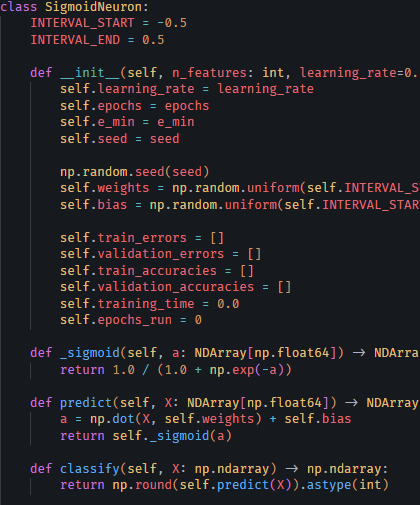
\includegraphics[width=0.75\linewidth]{2Lab/overleaf/images/SigmoidNeuron_Class_1.png}
    \caption{Sigmoidinio neurono klasės kodas 1 dalis}
    \label{fig:sigmoid_neuron_class_1}
\end{figure}

\begin{figure}[H]
    \centering
    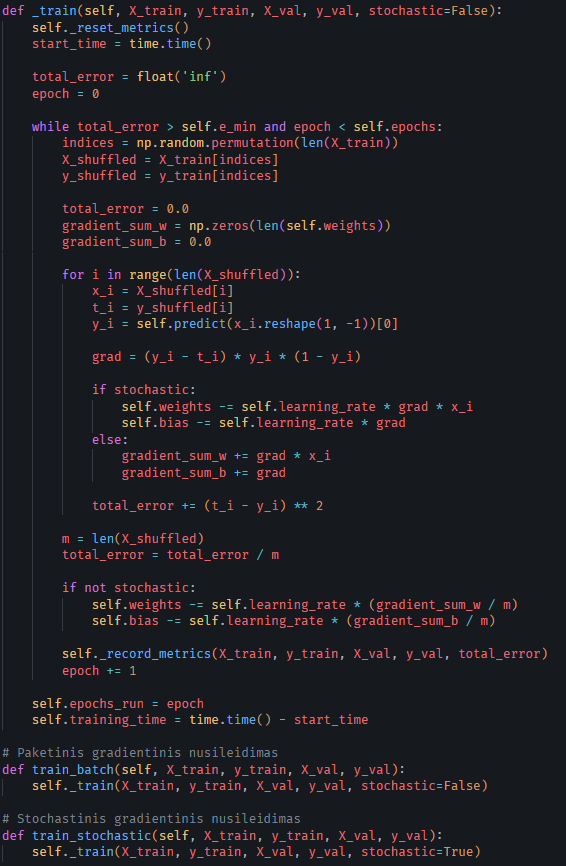
\includegraphics[width=0.75\linewidth]{2Lab/overleaf/images/SigmoidNeuron_Class_2.png}
    \caption{Sigmoidinio neurono klasės kodas 2 dalis}
    \label{fig:sigmoid_neuron_class_2}
\end{figure}

\begin{figure}[H]
    \centering
    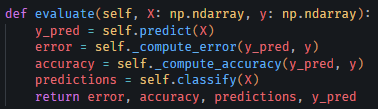
\includegraphics[width=0.75\linewidth]{2Lab/overleaf/images/SigmoidNeuron_Class_3.png}
    \caption{Sigmoidinio neurono klasės kodas 3 dalis}
    \label{fig:sigmoid_neuron_class_3}
\end{figure}